\documentclass[]{elsarticle} %review=doublespace preprint=single 5p=2 column
%%% Begin My package additions %%%%%%%%%%%%%%%%%%%
\usepackage[hyphens]{url}
\usepackage{lineno} % add
\providecommand{\tightlist}{%
  \setlength{\itemsep}{0pt}\setlength{\parskip}{0pt}}

\bibliographystyle{elsarticle-harv}
\biboptions{sort&compress} % For natbib
\usepackage{graphicx}
\usepackage{booktabs} % book-quality tables
%% Redefines the elsarticle footer
%\makeatletter
%\def\ps@pprintTitle{%
% \let\@oddhead\@empty
% \let\@evenhead\@empty
% \def\@oddfoot{\it \hfill\today}%
% \let\@evenfoot\@oddfoot}
%\makeatother

% A modified page layout
\textwidth 6.75in
\oddsidemargin -0.15in
\evensidemargin -0.15in
\textheight 9in
\topmargin -0.5in
%%%%%%%%%%%%%%%% end my additions to header

\usepackage[T1]{fontenc}
\usepackage{lmodern}
\usepackage{amssymb,amsmath}
\usepackage{ifxetex,ifluatex}
\usepackage{fixltx2e} % provides \textsubscript
% use upquote if available, for straight quotes in verbatim environments
\IfFileExists{upquote.sty}{\usepackage{upquote}}{}
\ifnum 0\ifxetex 1\fi\ifluatex 1\fi=0 % if pdftex
  \usepackage[utf8]{inputenc}
\else % if luatex or xelatex
  \usepackage{fontspec}
  \ifxetex
    \usepackage{xltxtra,xunicode}
  \fi
  \defaultfontfeatures{Mapping=tex-text,Scale=MatchLowercase}
  \newcommand{\euro}{€}
\fi
% use microtype if available
\IfFileExists{microtype.sty}{\usepackage{microtype}}{}
\usepackage{color}
\usepackage{fancyvrb}
\newcommand{\VerbBar}{|}
\newcommand{\VERB}{\Verb[commandchars=\\\{\}]}
\DefineVerbatimEnvironment{Highlighting}{Verbatim}{commandchars=\\\{\}}
% Add ',fontsize=\small' for more characters per line
\usepackage{framed}
\definecolor{shadecolor}{RGB}{248,248,248}
\newenvironment{Shaded}{\begin{snugshade}}{\end{snugshade}}
\newcommand{\KeywordTok}[1]{\textcolor[rgb]{0.13,0.29,0.53}{\textbf{{#1}}}}
\newcommand{\DataTypeTok}[1]{\textcolor[rgb]{0.13,0.29,0.53}{{#1}}}
\newcommand{\DecValTok}[1]{\textcolor[rgb]{0.00,0.00,0.81}{{#1}}}
\newcommand{\BaseNTok}[1]{\textcolor[rgb]{0.00,0.00,0.81}{{#1}}}
\newcommand{\FloatTok}[1]{\textcolor[rgb]{0.00,0.00,0.81}{{#1}}}
\newcommand{\ConstantTok}[1]{\textcolor[rgb]{0.00,0.00,0.00}{{#1}}}
\newcommand{\CharTok}[1]{\textcolor[rgb]{0.31,0.60,0.02}{{#1}}}
\newcommand{\SpecialCharTok}[1]{\textcolor[rgb]{0.00,0.00,0.00}{{#1}}}
\newcommand{\StringTok}[1]{\textcolor[rgb]{0.31,0.60,0.02}{{#1}}}
\newcommand{\VerbatimStringTok}[1]{\textcolor[rgb]{0.31,0.60,0.02}{{#1}}}
\newcommand{\SpecialStringTok}[1]{\textcolor[rgb]{0.31,0.60,0.02}{{#1}}}
\newcommand{\ImportTok}[1]{{#1}}
\newcommand{\CommentTok}[1]{\textcolor[rgb]{0.56,0.35,0.01}{\textit{{#1}}}}
\newcommand{\DocumentationTok}[1]{\textcolor[rgb]{0.56,0.35,0.01}{\textbf{\textit{{#1}}}}}
\newcommand{\AnnotationTok}[1]{\textcolor[rgb]{0.56,0.35,0.01}{\textbf{\textit{{#1}}}}}
\newcommand{\CommentVarTok}[1]{\textcolor[rgb]{0.56,0.35,0.01}{\textbf{\textit{{#1}}}}}
\newcommand{\OtherTok}[1]{\textcolor[rgb]{0.56,0.35,0.01}{{#1}}}
\newcommand{\FunctionTok}[1]{\textcolor[rgb]{0.00,0.00,0.00}{{#1}}}
\newcommand{\VariableTok}[1]{\textcolor[rgb]{0.00,0.00,0.00}{{#1}}}
\newcommand{\ControlFlowTok}[1]{\textcolor[rgb]{0.13,0.29,0.53}{\textbf{{#1}}}}
\newcommand{\OperatorTok}[1]{\textcolor[rgb]{0.81,0.36,0.00}{\textbf{{#1}}}}
\newcommand{\BuiltInTok}[1]{{#1}}
\newcommand{\ExtensionTok}[1]{{#1}}
\newcommand{\PreprocessorTok}[1]{\textcolor[rgb]{0.56,0.35,0.01}{\textit{{#1}}}}
\newcommand{\AttributeTok}[1]{\textcolor[rgb]{0.77,0.63,0.00}{{#1}}}
\newcommand{\RegionMarkerTok}[1]{{#1}}
\newcommand{\InformationTok}[1]{\textcolor[rgb]{0.56,0.35,0.01}{\textbf{\textit{{#1}}}}}
\newcommand{\WarningTok}[1]{\textcolor[rgb]{0.56,0.35,0.01}{\textbf{\textit{{#1}}}}}
\newcommand{\AlertTok}[1]{\textcolor[rgb]{0.94,0.16,0.16}{{#1}}}
\newcommand{\ErrorTok}[1]{\textcolor[rgb]{0.64,0.00,0.00}{\textbf{{#1}}}}
\newcommand{\NormalTok}[1]{{#1}}
\usepackage{longtable}
\usepackage{graphicx}
% We will generate all images so they have a width \maxwidth. This means
% that they will get their normal width if they fit onto the page, but
% are scaled down if they would overflow the margins.
\makeatletter
\def\maxwidth{\ifdim\Gin@nat@width>\linewidth\linewidth
\else\Gin@nat@width\fi}
\makeatother
\let\Oldincludegraphics\includegraphics
\renewcommand{\includegraphics}[1]{\Oldincludegraphics[width=\maxwidth]{#1}}
\ifxetex
  \usepackage[setpagesize=false, % page size defined by xetex
              unicode=false, % unicode breaks when used with xetex
              xetex]{hyperref}
\else
  \usepackage[unicode=true]{hyperref}
\fi
\hypersetup{breaklinks=true,
            bookmarks=true,
            pdfauthor={},
            pdftitle={Homework 2: NRSG 741},
            colorlinks=true,
            urlcolor=blue,
            linkcolor=magenta,
            pdfborder={0 0 0}}
\urlstyle{same}  % don't use monospace font for urls
\setlength{\parindent}{0pt}
\setlength{\parskip}{6pt plus 2pt minus 1pt}
\setlength{\emergencystretch}{3em}  % prevent overfull lines
\setcounter{secnumdepth}{0}
% Pandoc toggle for numbering sections (defaults to be off)
\setcounter{secnumdepth}{0}
% Pandoc header


\usepackage[nomarkers]{endfloat}

\begin{document}
\begin{frontmatter}

  \title{Homework 2: NRSG 741}
    \author[Emory University]{Tommy Flynn\corref{c1}}
   \ead{tjflynn@emory.edu} 
   \cortext[c1]{Corresponding Author}
      \address[Emory University]{Emory School of Nursing 1520 Clifton Rd Atlanta GA 30322}
  
  \begin{abstract}
  This assignment applies the dplyr and ggplot2 packages to work with the
  Davis dataset in the car package, which contains data on the measured
  and reported heights and weights of men and women engagedin regular
  exercise. The associated GitHub repository can be found at
  \url{https://github.com/tommyflynn/N741_Homework/tree/master/Flynn_HW_02}.
  \end{abstract}
  
 \end{frontmatter}

\subparagraph{1. What kind of R object is the Davis
dataset?}\label{what-kind-of-r-object-is-the-davis-dataset}

\begin{Shaded}
\begin{Highlighting}[]
\NormalTok{davis <-}\StringTok{ }\NormalTok{car::Davis}
\CommentTok{# to print class inline, use `r paste(class(davis))` Q2: to print number of}
\CommentTok{# observations, use `r count(davis)`}
\end{Highlighting}
\end{Shaded}

\begin{quote}
Answer: The Davis dataset is the ``data.frame'' class of R object.
\end{quote}

\subparagraph{2. How many observations are in the Davis
dataset?}\label{how-many-observations-are-in-the-davis-dataset}

\begin{quote}
Answer: There are 200 observations.
\end{quote}

\subparagraph{3. For reported weight, how many observations have a
missing
value?}\label{for-reported-weight-how-many-observations-have-a-missing-value}

\begin{Shaded}
\begin{Highlighting}[]
\CommentTok{# Use the is.na function to filter non-missing values from the repwt}
\CommentTok{# variable, then show inline with `r count(repmissing)`}
\NormalTok{repmissing <-}\StringTok{ }\KeywordTok{filter}\NormalTok{(davis, }\KeywordTok{is.na}\NormalTok{(repwt))}
\end{Highlighting}
\end{Shaded}

\begin{quote}
Answer: Reported weight has 17 missing values
\end{quote}

\subparagraph{4. How many observations have missing
values?}\label{how-many-observations-have-missing-values}

\begin{Shaded}
\begin{Highlighting}[]
\CommentTok{# HINT: find the complete rows... then show inline with `r completeobs`}
\NormalTok{completeobs <-}\StringTok{ }\KeywordTok{count}\NormalTok{(}\KeywordTok{na.omit}\NormalTok{(davis))}
\end{Highlighting}
\end{Shaded}

\begin{quote}
Answer: The Davis dataset has 181 complete observations.
\end{quote}

\subparagraph{5. Create a subset containing only females. How many
females are in this
subset?}\label{create-a-subset-containing-only-females.-how-many-females-are-in-this-subset}

\begin{Shaded}
\begin{Highlighting}[]
\CommentTok{# create a subset of all female obs, print #obs inline with `r}
\CommentTok{# count(femaleset)}
\NormalTok{femaleset <-}\StringTok{ }\NormalTok{davis %>%}\StringTok{ }\KeywordTok{subset}\NormalTok{(sex ==}\StringTok{ "F"}\NormalTok{)}
\end{Highlighting}
\end{Shaded}

\begin{quote}
Answer: A subset containing only females from the Davis data has 112
observations.
\end{quote}

\subparagraph{6. What is the average BMI for these
individuals?}\label{what-is-the-average-bmi-for-these-individuals}

\begin{Shaded}
\begin{Highlighting}[]
\CommentTok{# create a new data.fram with height unit transformation (cm -> m),}
\CommentTok{# calculated BMI, and categorized BMI.}
\NormalTok{davisBMI <-}\StringTok{ }\NormalTok{davis %>%}\StringTok{ }\KeywordTok{mutate}\NormalTok{(}\DataTypeTok{sqrmetHT =} \NormalTok{(height/}\DecValTok{100}\NormalTok{) *}\StringTok{ }\NormalTok{(height/}\DecValTok{100}\NormalTok{)) %>%}\StringTok{ }\KeywordTok{mutate}\NormalTok{(}\DataTypeTok{BMI =} \NormalTok{weight/sqrmetHT) %>%}\StringTok{ }
\StringTok{    }\KeywordTok{mutate}\NormalTok{(}\DataTypeTok{BMIclass =} \KeywordTok{if_else}\NormalTok{(BMI <}\StringTok{ }\FloatTok{18.5}\NormalTok{, }\StringTok{"1. Underweight"}\NormalTok{, }\KeywordTok{if_else}\NormalTok{(BMI <}\StringTok{ }\DecValTok{25}\NormalTok{, }
        \StringTok{"2. Normal"}\NormalTok{, }\KeywordTok{if_else}\NormalTok{(BMI <}\StringTok{ }\DecValTok{30}\NormalTok{, }\StringTok{"3. Overweight"}\NormalTok{, }\StringTok{"4. Obese"}\NormalTok{, }\StringTok{"Missing"}\NormalTok{), }
        \StringTok{"Missing"}\NormalTok{)))}
\CommentTok{# Print for Q6 inline with, `r mean(davisBMI$BMI)`}
\end{Highlighting}
\end{Shaded}

\begin{quote}
Answer: The mean BMI is 24.7009556.
\end{quote}

\subparagraph{7. How do these individuals fall into the BMI categories
(what are the frequencies and relative
\%'s)?}\label{how-do-these-individuals-fall-into-the-bmi-categories-what-are-the-frequencies-and-relative-s}

\begin{Shaded}
\begin{Highlighting}[]
\CommentTok{# Use janitor tably() and knitr kable() functions to make it pretty}
\NormalTok{davisBMI %>%}\StringTok{ }\NormalTok{janitor::}\KeywordTok{tabyl}\NormalTok{(BMIclass) %>%}\StringTok{ }\NormalTok{knitr::}\KeywordTok{kable}\NormalTok{()}
\end{Highlighting}
\end{Shaded}

\begin{longtable}[]{@{}lrr@{}}
\toprule
BMIclass & n & percent\tabularnewline
\midrule
\endhead
1. Underweight & 18 & 0.090\tabularnewline
2. Normal & 143 & 0.715\tabularnewline
3. Overweight & 35 & 0.175\tabularnewline
4. Obese & 4 & 0.020\tabularnewline
\bottomrule
\end{longtable}

\section{Graphs with ggplot2}\label{graphs-with-ggplot2}

\subparagraph{8. Create a histogram of
BMI.}\label{create-a-histogram-of-bmi.}

\begin{Shaded}
\begin{Highlighting}[]
\NormalTok{davisBMI %>%}\StringTok{ }\KeywordTok{filter}\NormalTok{(!}\KeywordTok{is.na}\NormalTok{(BMI)) %>%}\StringTok{ }\KeywordTok{filter}\NormalTok{(BMI <}\StringTok{ }\DecValTok{50}\NormalTok{) %>%}\StringTok{ }\KeywordTok{ggplot}\NormalTok{(}\KeywordTok{aes}\NormalTok{(BMI), }\DataTypeTok{show.legend =} \OtherTok{FALSE}\NormalTok{, }
    \DataTypeTok{caption =} \StringTok{"BMI Histogram"}\NormalTok{) +}\StringTok{ }\KeywordTok{geom_histogram}\NormalTok{(}\KeywordTok{aes}\NormalTok{(}\DataTypeTok{y =} \NormalTok{..density..), }\DataTypeTok{colour =} \StringTok{"black"}\NormalTok{, }
    \DataTypeTok{fill =} \StringTok{"yellow"}\NormalTok{, }\DataTypeTok{position =} \StringTok{"dodge"}\NormalTok{, }\DataTypeTok{binwidth =} \DecValTok{1}\NormalTok{) +}\StringTok{ }\KeywordTok{geom_density}\NormalTok{(}\DataTypeTok{alpha =} \FloatTok{0.2}\NormalTok{, }
    \DataTypeTok{fill =} \StringTok{"blue"}\NormalTok{)}
\end{Highlighting}
\end{Shaded}

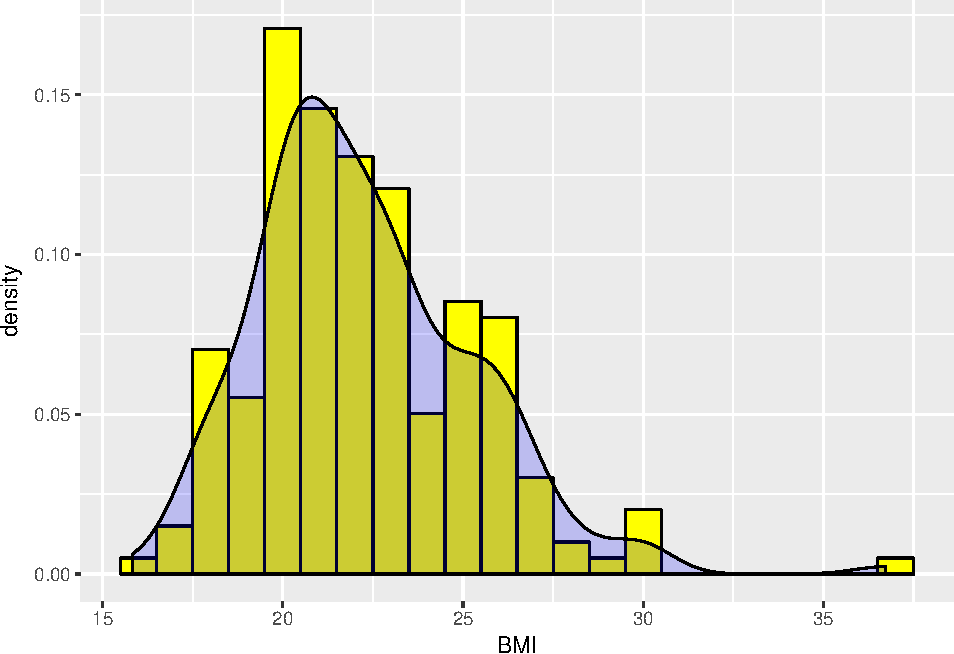
\includegraphics{Flynn_HW_02_files/figure-latex/histogram BMI-1.pdf}

\end{document}


